% !TeX spellcheck = ru_RU
% !TEX root = vkr.tex

\section{Подробности реализации}

В качестве языка реализации проекта был выбран \Haskell{}.
Предполагаемая архитектура изображена на рисунке~\ref{fig:lmlcmods}.

Для сборки проекта и версионирования зависимостей используется \textsc{Stack}\footnote{Сайт проекта: \url{https://docs.haskellstack.org/en/stable/} (дата обращения \DTMdate{2025-02-25})}, каждая часть, описанная в разделе~\ref{sec:big-arch}, является отдельным пакетом.
Для тестирования используется фреймворк \textsc{Tasty}\footnote{Описание проекта на \textsc{Hackage}: \url{https://hackage.haskell.org/package/tasty/} (дата обращения \DTMdate{2025-02-25})}, по умолчанию все части компилятора покрываются golden\footnote{Описание golden тестов: \url{https://ro-che.info/articles/2017-12-04-golden-tests} (дата обращения \DTMdate{2025-02-25})} тестами.

\begin{figure}[h]
    \begin{center}
        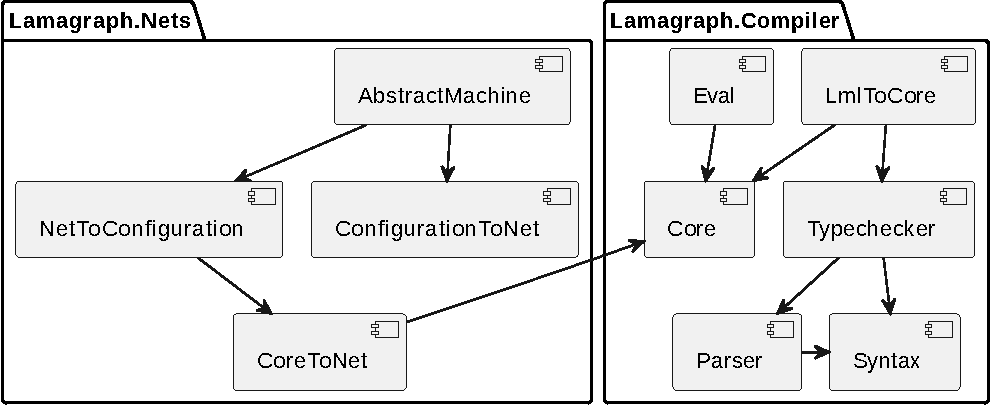
\includegraphics{components}
    \end{center}
    \caption{Архитектура транслятора}
    \label{fig:lmlcmods}
\end{figure}

\paragraph{Синтаксис языка.}

Синтаксис языка основан на \OCaml{}.
Однако упрощен для простоты реализации\footnote{С полной грамматикой можно ознакомиться в репозитории проекта: \url{https://github.com/Lamagraph/interaction-nets-in-fpga/blob/main/lamagraph-compiler/src/Lamagraph/Compiler/Syntax.hs} (дата обращения \DTMdate{2025-02-25})}.
Так, например в языке остались стандартные для функциональных языков конструкции, такие как сопоставление с образцом, рекурсивные и взаимнорекурсивные функции, а также алгебраические типы данных.
Однако в отличие от \OCaml{} отсутствует поддержка классов и функторов, а система модулей максимально упрощена и напоминает систему модулей в F\#.

Для представления AST (дерева абстрактного синтаксиса) используется паттерн Trees That Grow (TTG)~\cite{shayannajdTreesThatGrow}.
Он позволяет с помощью механизма type families~\cite{schrijversTypeCheckingOpen2008} гибко параметризовать дерево необходимыми аннотациями, более того аннотации могут различаться в разных узлах дерева, тем самым поддерживая безопасность кода.

\paragraph{Парсер.}

Для синтаксического анализа используется связка лексера \textsc{Alex} и парсер-генератора \textsc{Happy}, которые являются аналогами \textsc{flex} и \textsc{bison}, написанными на \Haskell{}.

На данном этапе аннотации с помощью TTG не используются.

Для тестирования лексера используются модульные тесты.
Для парсера используется property-based тестирование с использованием библиотеки \textsc{Hedgehog}\footnote{Репозиторий проекта: \url{https://github.com/hedgehogqa/haskell-hedgehog/} (дата обращения: \DTMdate{2025-02-19})}.
Данный метод основан на том, что синтаксический анализ в AST и печать AST должны давать тождественное отображение при композиции.

\paragraph{Вывод типов.}

Поскольку язык ML-подобный, используется система типов Хиндли-Милнера~\cite{hindleyPrincipalTypeSchemeObject1969, milnerTheoryTypePolymorphism1978}.

На данном этапе в аннотациях TTG сохраняется тип каждого узла дерева.

\paragraph{Промежуточное представление.}

AST получаемый после парсинга и вывода типов получается достаточно сложным~--- в нём большое количество различных узлов с аннотациями.
Для упрощения дальнейшей работы используется промежуточное представление на основе GHC Core\footnote{Подробнее можно прочитать по ссылке: \url{https://gitlab.haskell.org/ghc/ghc/-/wikis/commentary/compiler/core-syn-type} (дата обращения: \DTMdate{2025-02-19})}, также часто называемое обогащённым $\lambda$-исчислением\footnote{Подробнее узнать про способы обогащения $\lambda$-исчисления можно в~\cite[раздел~3.2]{peytonjones1987the}}.
Его описание представлено на листинге~\ref{lst:core}.

\begin{listing}
    \inputminted[fontsize=\footnotesize]{haskell}{figures/core.hs}
    \caption{Представление Core в алгебраических типах данных.}
    \label{lst:core}
\end{listing}

Важными отличиями от GHC Core являются наличие выделенного конструктора для пар, а также отсутствие типизации.

Наличие выделенного конструктора для пар обусловлено различием между ML и \Haskell{}~--- в первом пары тоже выделены и могут быть какой угодно арности, во втором же пара является синтаксическим сахаром для алгебраического типа-суммы и ограничена арностью 63.

От типизации пришлось отказаться в угоду простоты реализации, а также в виду отсутствия оптимизаций со стороны компилятора, где наличие типов упрощает и делает более безопасным их применение.

\paragraph{Трансляция высокоуровневого AST в промежуточное представление.}

Алгоритм трансляции достаточно прямолинеен, наиболее сложной частью является трансляция сложных шаблонов в левой части let-связывания и замена вложенных шаблонов на вложенные match-выражения.
